%%%%%%%%%%%%%%%%%%%%%%%%%%%%%%%%%%%%%%%%%%%%%%%%%%%%%%%%%%%%%%%%%%%%%%%%%%%%%
%%% LaTeX-Rahmen fuer das Erstellen von Masterarbeiten
%%%%%%%%%%%%%%%%%%%%%%%%%%%%%%%%%%%%%%%%%%%%%%%%%%%%%%%%%%%%%%%%%%%%%%%%%%%%%

%%%%%%%%%%%%%%%%%%%%%%%%%%%%%%%%%%%%%%%%%%%%%%%%%%%%%%%%%%%%%%%%%%%%%%%%%%%%%
%%% allgemeine Einstellungen
%%%%%%%%%%%%%%%%%%%%%%%%%%%%%%%%%%%%%%%%%%%%%%%%%%%%%%%%%%%%%%%%%%%%%%%%%%%%%

\documentclass[twoside,12pt,a4paper]{report}
%\usepackage{reportpage}
\usepackage{epsf}
\usepackage{graphics, graphicx}
\usepackage{latexsym}
\usepackage[margin=10pt,font=small,labelfont=bf]{caption}
\usepackage[utf8]{inputenc}
\usepackage[toc,page]{appendix}
\usepackage[acronym,nomain]{glossaries} % list of abbreviations
\usepackage{amsmath} %type math formulars
\usepackage[]{algorithm2e}% wirte pseudcocode
\usepackage{float} % set picture at exact location
\usepackage{amssymb} %math symbols

\textwidth 14cm
\textheight 22cm
\topmargin 0.0cm
\evensidemargin 1cm
\oddsidemargin 1cm
%\footskip 2cm
\parskip0.5explus0.1exminus0.1ex

% Kann von Student auch nach pers\"onlichem Geschmack ver\"andert werden.
\pagestyle{headings}
\makeglossaries
\sloppy

\begin{document}

%%%%%%%%%%%%%%%%%%%%%%%%%%%%%%%%%%%%%%%%%%%%%%%%%%%%%%%%%%%%%%%%%%%%%%%%%%%%
%%% hier steht die neue Titelseite 
%%%%%%%%%%%%%%%%%%%%%%%%%%%%%%%%%%%%%%%%%%%%%%%%%%%%%%%%%%%%%%%%%%%%%%%%%%%%
 
\begin{titlepage}
 \begin{center}
  {\LARGE Eberhard Karls Universit\"at T\"ubingen}\\
  {\large Mathematisch-Naturwissenschaftliche Fakult\"at \\
Wilhelm-Schickard-Institut f\"ur Informatik\\[4cm]}
  {\huge Master Thesis Bioinformatics\\[2cm]}
  {\Large\bf  Title of thesis\\[1.5cm]}
 {\large Vor- und Nachname}\\[0.5cm]
Datum\\[4cm]
{\small\bf Reviewers}\\[0.5cm]
  \parbox{7cm}{\begin{center}{\large Name Erstgutachter}\\
   (Bioinformatik)\\
  {\footnotesize Wilhelm-Schickard-Institut f\"ur Informatik\\
	Universit\"at T\"ubingen}\end{center}}\hfill\parbox{7cm}{\begin{center}
  {\large Name Zweitgutachter}\\
  (Biologie/Medizin)\\
  {\footnotesize Medizinische Fakult\"at\\
	Universit\"at T\"ubingen}\end{center}
 }
  \end{center}
\end{titlepage}

%%%%%%%%%%%%%%%%%%%%%%%%%%%%%%%%%%%%%%%%%%%%%%%%%%%%%%%%%%%%%%%%%%%%%%%%%%%%
%%% Titelr"uckseite: Bibliographische Angaben
%%%%%%%%%%%%%%%%%%%%%%%%%%%%%%%%%%%%%%%%%%%%%%%%%%%%%%%%%%%%%%%%%%%%%%%%%%%%

\thispagestyle{empty}
\vspace*{\fill}
\begin{minipage}{11.2cm}
\textbf{Nachname, Vorname:}\\
\emph{Title of thesis}\\ Master Thesis Bioinformatics\\
Eberhard Karls Universit\"at T\"ubingen\\
Thesis period: von-bis
\end{minipage}
\newpage

%%%%%%%%%%%%%%%%%%%%%%%%%%%%%%%%%%%%%%%%%%%%%%%%%%%%%%%%%%%%%%%%%%%%%%%%%%%%

\pagenumbering{roman}
\setcounter{page}{1}

%%%%%%%%%%%%%%%%%%%%%%%%%%%%%%%%%%%%%%%%%%%%%%%%%%%%%%%%%%%%%%%%%%%%%%%%%%%%
%%% Seite I: Zusammenfassug, Danksagung
%%%%%%%%%%%%%%%%%%%%%%%%%%%%%%%%%%%%%%%%%%%%%%%%%%%%%%%%%%%%%%%%%%%%%%%%%%%%


\section*{Abstract}

Write here your abstract.
\newpage
\section*{Zusammenfassung}

Bei einer englischen Masterarbeit muss zus\"atzlich eine deutsche Zusammenfassung verfasst werden.

\newpage
\section*{Acknowledgements}

Write here your acknowledgements.

\cleardoublepage

%%%%%%%%%%%%%%%%%%%%%%%%%%%%%%%%%%%%%%%%%%%%%%%%%%%%%%%%%%%%%%%%%%%%%%%%%%%%%
%%% Table of Contents
%%%%%%%%%%%%%%%%%%%%%%%%%%%%%%%%%%%%%%%%%%%%%%%%%%%%%%%%%%%%%%%%%%%%%%%%%%%%%

\renewcommand{\baselinestretch}{1.3}
\small\normalsize

\tableofcontents

\renewcommand{\baselinestretch}{1}
\small\normalsize

\cleardoublepage

%%%%%%%%%%%%%%%%%%%%%%%%%%%%%%%%%%%%%%%%%%%%%%%%%%%%%%%%%%%%%%%%%%%%%%%%%%%%%
%%% List of Figures
%%%%%%%%%%%%%%%%%%%%%%%%%%%%%%%%%%%%%%%%%%%%%%%%%%%%%%%%%%%%%%%%%%%%%%%%%%%%%

\renewcommand{\baselinestretch}{1.3}
\small\normalsize

\addcontentsline{toc}{chapter}{List of Figures}
\listoffigures

\renewcommand{\baselinestretch}{1}
\small\normalsize

\cleardoublepage

%%%%%%%%%%%%%%%%%%%%%%%%%%%%%%%%%%%%%%%%%%%%%%%%%%%%%%%%%%%%%%%%%%%%%%%%%%%%%
%%% List of tables
%%%%%%%%%%%%%%%%%%%%%%%%%%%%%%%%%%%%%%%%%%%%%%%%%%%%%%%%%%%%%%%%%%%%%%%%%%%%%

\renewcommand{\baselinestretch}{1.3}
\small\normalsize

\addcontentsline{toc}{chapter}{List of Tables}
\listoftables

\renewcommand{\baselinestretch}{1}
\small\normalsize

\cleardoublepage

%%%%%%%%%%%%%%%%%%%%%%%%%%%%%%%%%%%%%%%%%%%%%%%%%%%%%%%%%%%%%%%%%%%%%%%%%%%%%
%%% List of abbreviations
%%%%%%%%%%%%%%%%%%%%%%%%%%%%%%%%%%%%%%%%%%%%%%%%%%%%%%%%%%%%%%%%%%%%%%%%%%%%%

\printglossaries
\newacronym{ea}{EA}{Evolutionary Algorithm}
\newacronym{neat}{NEAT}{Neuroevolution Of Augmenting Toplogies}
\newacronym{hyperNEAT}{HyperNEAT}{Hypercube-based NeuroEvolution of Aug
menting Topologies}
\newacronym{EShyperNEAT}{ES-HyperNEAT}{Evolvable Substrate Hypercube-based NeuroEvolution of Aug
	menting Topologies}
\newacronym{cppn}{CPPN}{Compositional Pattern Producing Network CPPN}
\newacronym{ann}{ANN}{Artificial Neural Network}
%\addcontentsline{toc}{chapter}{List of Abbreviations}
%\chapter*{List of Abbreviations\markboth{LIST OF ABBREVIATIONS}{LIST OF ABBREVIATIONS}}
%
%\begin{tabbing}
%\textbf{FACTOTUM}\hspace{1cm}\=Schrott\kill
%\textbf{BLAST}\>Basic Local Alignment Search Tool \\
%\textbf{...} \> ...\\
%\end{tabbing}

\cleardoublepage

%%%%%%%%%%%%%%%%%%%%%%%%%%%%%%%%%%%%%%%%%%%%%%%%%%%%%%%%%%%%%%%%%%%%%%%%%%%%%
%%% Der Haupttext, ab hier mit arabischer Numerierung
%%% Mit \input{dateiname} werden die Datei `dateiname' eingebunden
%%%%%%%%%%%%%%%%%%%%%%%%%%%%%%%%%%%%%%%%%%%%%%%%%%%%%%%%%%%%%%%%%%%%%%%%%%%%%

\pagenumbering{arabic}
\setcounter{page}{1}

%%%%%%%%%%%%%%%%%%%%%%%%%%%%%%%%%%%%%%%%%%%%%%%%%%%%%%%%%%%%%%%%%%%%
% Basic Informations
%%%%%%%%%%%%%%%%%%%%%%%%%%%%%%%%%%%%%%%%%%%%%%%%%%%%%%%%%%%%%%%%%%%%

\chapter{Fundamentals}\label{Basics}
\section{TODO}
-> neural networks
ANN: 
SNN:


\section{NEAT}\label{NEAT} % todo in ea section packen... und mit em deitschen ea paper zitieren. Biologisch eh nicht ganz korrekt
\Gls{neat} (\cite{NEAT}) is an neuroevolution method that genetically encodes and evolves weights and topologies of neural networks. \gls{neat} stands out from other neuroevolution algorithms by meaningful crossovers in disparate ANN topologies, protection of topological innovations and a efficient search by a stepwise increasing search space. (TODO cite some). Furthermore \gls{neat} is well suited for reinforcement learning problems. 

\subsection{Evolutionary algorithm} % Todo abkürzung EA
Evolutionary algorithms (EAs) (see generally \cite{book:IntroductionEA},\cite{book:IntroductionEA}) are algorithms that mimic the natural evolution process. That is simplified in a way that only fittest organisms of a generation will survive. An EA maintains a group of solutions called a population. A solution in a population is called an individual. Each individual has a numerical fitness value that determines how good this solution is. An individual is represented by a code also called genome. A genome consists of multiply genes. Genes are responsible for expressing specific feature. Genes that express same features with different characteristics are called alleles. During the run of an EA a genome of an individual undergoes several variation operations. One typical operations are mutations, where parts of the genome are changed randomly. Cross Over as an other typical operation exchanges parts of the genome of two individuals. Usually an EA performs those operations to generations and only the fittest children are taken over into a new generation. The function giving the fitness of an individual is called objective function. EAs are mainly used to find good local maxima of objective functions that are either unknown or not analytical differentiable and not solvable with numerical methods like gradient descends.  (TODO nachlesen vergleichn script zell). A  typical EA solution process can be illustrated as follows:
%\begin{algorithm}
%	\LinesNumbered
	\SetCommentSty{text} 
\begin{algorithm}[h!] % or H with float
   \TitleOfAlgo{Exemplar EA}
	choose strategy parameters\;
	create initial population P(0)\;
	$t \gets 0$\;
	evaluate fitness of the initial population\;
	\While{termination condition not reached}{
		$t \gets t+1$\;
		apply variation operations \tcp*[r]{e.g. mutation, cross over}
	    evaluate fitness of new individuals\;
		create new population P(t)\;
	}
 	output results;
 	
	%\caption{How to write algorithms}
\end{algorithm}
%\end{algorithm}...
TODO typischer evolutionszykel erklären.


\subsection{operating principle} 
The genetic basic of \gls{neat} is a direct encoded genome, which contains connection and node genes. Each node gene evolves a neuron while each connection gene represents a weighted and directed connection between two neurons. A node gene contains it's identification number and it's type. Possible types are Input, Output and Hidden. A connection gene encodes its connection by referring to two node gene identification numbers. In addition a connection gene contains its weight, an expression flag and an innovation number. The expression flag indicates whether the expression gets realised or not. The innovation number is the fixed identification number of a connection gene. Alleles of a connection gene share the same node genes and innovation number but can have different weight and expression flag values. Every time a new neuron gene or connection gene is created a global counter number is increased by one and than used as the new innovation number. In the case that the same connection gets created in two different offsprings of a generation they get the same innovation number assigned. This only applies if it happens in the same generation. Thus one gene can only evolve in one particular generation. As a result the innovation number assures that connection genes with the same innovation number connect the same nodes but not all connection genes connecting the same nodes have the same connection number.(this represents the biological fact, that the same feature can be expressed by different genes.). An example for a NEAT genome is depicted in figure \ref{fig:neatgenome}.\\
Three types of mutation are realized. A \textit{weight mutation} mutates each weight mutates with the same probability. New connections are added by the add connection mutation. Thereby two unconnected cells are randomly chosen and connected by a new connection gene with a random weight. A new cell mutation splits an existing connection by placing a new node between the two former connected nodes. This is realized by disabling the old connection gene and the creation of two new connection genes and one new node gene. One connection gene connects the input node with the new node and gets its weight set to the value of the former connection. The other connection gene is connects the new node with the output node of the former connection and gets its weight set to one. This expression of weights leads to an minimized initial effect of a mutation. Two exemplar mutations are displayed in figure \ref{fig:neatmutations}.\\
In? a cross over at first a synapsis is done. This means that all connection genes of two individuals are lined up. Genes that have the same innovation number are called matching genes. Genes of one individual which innovation numbers are inside the range of the other individual matching genes' innovation numbers are called disjoint genes. Innovation numbers outside the range of the other individual matching genes' innovation numbers are called excess genes. The child's genome is created by selecting one gene randomly out of each tuple of matching genes, disjoint and access genes are taken from the more fit parent. With a preset probability a disabled gene can be enabled again when it is disabled in both parents. By crossing over only connections and no whole substructures of the network (like other approaches do  TODO find one vorlesung Zell trees), it is ensured that a new proper artificial neural network is created. 
An exemplar cross over of two individuals with the same fitness is shown in figure \ref{fig:neatcrossover}. \\
Specitation: 
Based on empirical evidence insertion of new structures into a network leads at first to a decrease in fitness. Thus its unlikely that the individual can compete against others in this generation and will be distinct. A new structure needs some time to adapt its weights in a way that the new structure is beneficial. Thus specitation also known as niching is implemented in NEAT to protect new structure. Similar individuals are put in their own species. Members of a species are primarily competing against each others. That means artificial neural networks with similar structures are primarily competing against each other. To determine to which species an individual belongs the following distance measurement between two aligned individuals is used:
\begin{equation*} 
\delta = \dfrac{c_1E}{N}+\dfrac{c_2D}{N}+c_3*\overline{W}.
\end{equation*}
Where $E$ is the number of excess genes and $D$ the number of disjoint genes. $\overline{W}$ is the average of weight differences of all matching genes. The normalization factor $N$ is the number of genes of the larger genome. $c_1$,$c_2$,$c_3$ represent scaling factors. 
In detail a ordered list of species is given. For the next generation one representative individual is randomly chosen out of each species. Each member $m$ of the next generation is compared consecutively to these representatives. If the distance measurement $\delta$ is smaller than a fixed threshold $\delta_t$, $m$ is put into the species of the representative. If $m$ is not compatible to any representative a new species with $m$ as its representative is created. This way assures disjunct species.
To prevent that one species takes over the entire population explicit fitness sharing (TODO link Golsberg and Richardson 1987) is used. For each individual $i$ its adjusted fitness $f_{i}^{'}$ is calculated the following way:
\begin{align*} 
f_{i}^{'}&=\dfrac{f_i}{\displaystyle\sum_{j=1}^{n} sh(\delta(i,j)) }\\
sh(i,j) &= \begin{cases}
1 & \quad \text{if } \delta(i,j) < \delta_t \\
0 & \quad \text{if } \delta(i,j) \geq \delta_t
\end{cases}
\end{align*}
Where $f_i$ is the fitness of $i$, $\delta(i,j)$ the distance between individual $i$ and $j$. And $sh$ a sharing function that determines whether $i$ and $j$ are in the same species.
As a result under the assumption that the fitness function has no plateaus at local maxima the shared fitness of species members is decreased if the species gets larger. Every species produces a number of offsprings $NO$ proportional to the sum of adjusted fitnesses $f_{i}^{'}$ of its members. The total amount of offsprings is limited by the maximum population size $P$ and the number of individuals that are taken over directly from the last generation $L$.
\begin{equation*} 
NO(s) = (P-L)\cdot\dfrac{\displaystyle\sum_{\forall i \in s} f_{i}^{'}}{\displaystyle\sum_{\forall i } f_{i}^{'}}
\end{equation*}
  %TODO bei zell im script nachlesen -> verbessern.
\\ NEAT starts with a minimal structure. That is, each input neuron and one optional bias neuron is connected with each output neuron. There are no hidden neurons. Starting with a minimal structure leads to an efficient search. Since add node mutations and add connection mutations are rare compared to weight mutations the search space is increased slowly. The search space consists of one dimension for each weight and one dimension representing the number of neurons. That means starting with a minimal network networks with increasing complexity are considered as solution for the problem.


 
  
  
\begin{figure}[tb]
	\centering
	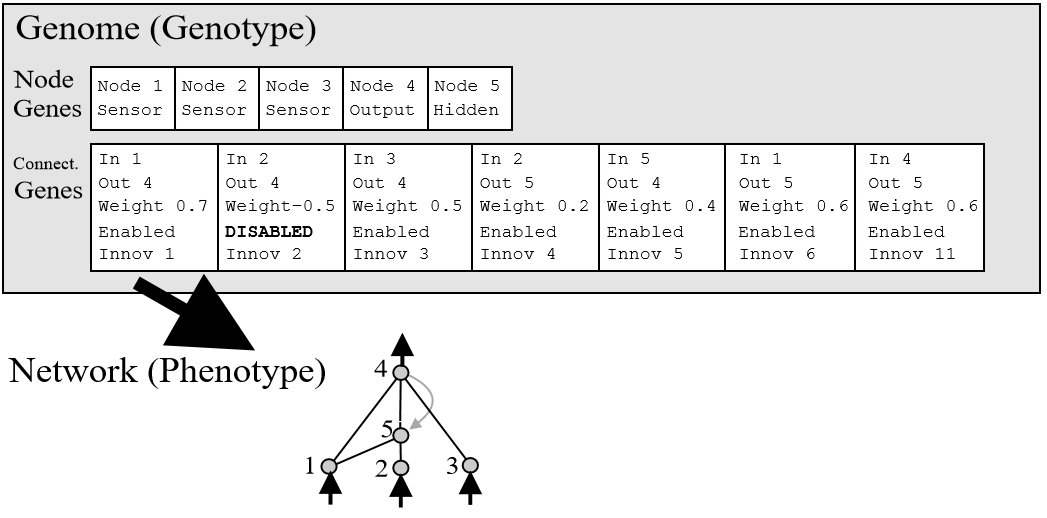
\includegraphics[width=0.7\linewidth]{figures/NEAT/NEATGenome}
	\caption[NEAT genome]{NEAT genomes consist of two type of genes: node genes displayed in the first row and connection genes displayed in the second row. Each node gene has an identification number (first element) and one of three types: sensor (input), output and hidden. A connection gene contains its input and output node, a weight, an expression flag and a innovation number. Underneath the genome the resulting network is displayed. The numbers are identical to the node IDs. Enabled connections are displayed black. Disabled connections are shown grey. \cite[p. 106]{NEAT} }
	\label{fig:neatgenome} % TODO wirklich so ausführlich wiederholen notwendig?
\end{figure}
  
  
  
\begin{figure}[tb]
	\centering
	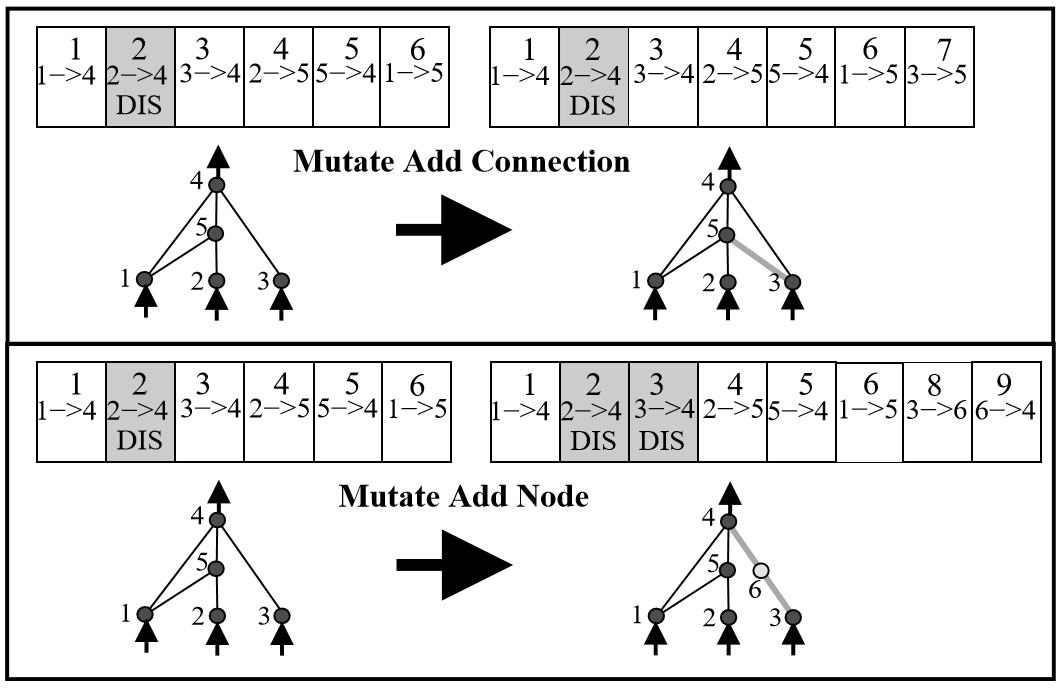
\includegraphics[width=0.7\linewidth]{figures/NEAT/NEATMutations}
	\caption[NEAT mutations]{At the top a add connection mutation is displayed. The unconnected nodes 3 and 5 are chosen randomly. Then a connection gene between  those nodes is created. The global innovation counter number is increased by one (from 6 to 7) and allied to the new connection gene.\\
	At the bottom a add node mutation is displayed. Connection 3 is randomly chosen and gets disabled. Next a new node gene with ID 6 is created. Then fist new connection gene connecting  node 3 and 6 with innovation number 8 and a second connecting node 6 and 4 with innovation number 9 is created. \\
Note that only connection genes are displayed. The top number in each gene is its innovation number followed by the node it connects and the expression flag.
Node genes are not depicted.
\cite[p. 107]{NEAT}}
	\label{fig:neatmutations}
\end{figure}
  
  
  
\begin{figure}[tb]
	\centering
	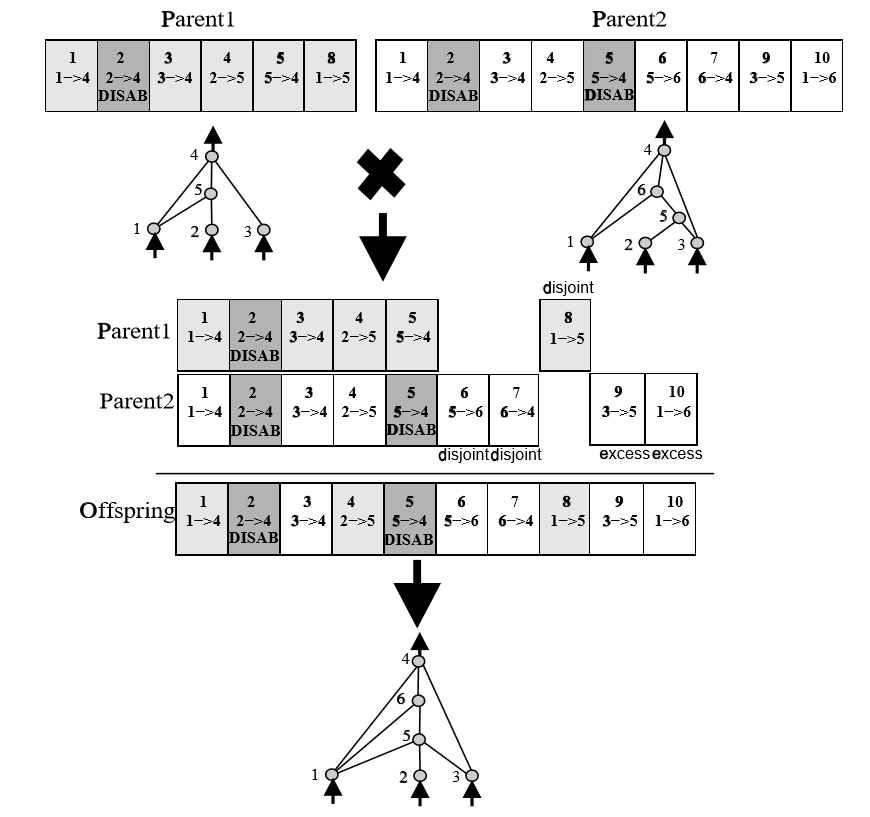
\includegraphics[width=0.7\linewidth]{figures/NEAT/NEATCrossOver}
	\caption[NEAT cross over]{Two individual's connection genes and their corresponding networks are displayed at the top. Underneath this two genomes got aligned. All connection genes with same innovation numbers are displayed opposite each other. Those are matching genomes. All connection genes of one individual that are in the range of the other individual's connection gene are marked as disjoint. Connection genes that are outside the range of the other individual's connection gene are marked are marked as excess. The offspring's connection gene consists of one randomly chosen connection gene out of each matching gene. In this example the fitness of both parent individuals is equal. Thus all excess and disjoint connection genes are chosen. If the fitnesses would differ the excess and disjoint connection of the more fit parent are taken over.\cite[p. 109]{NEAT}}
	\label{fig:neatcrossover}
\end{figure}
  
  
Neuroevolution is a machine learning technique that evolves weights and topology of artificial neural networks by means of evolutionary algorithms. 

TODO: explain 
Neuroevolution
evolutionary algorithm


"Neuro-evolution of augmenting topologies (NEAT) is a method for genetically encoding and evolving the architecture and the weights of neural networks "

\section{HyperNEAT}\label{HYPERNEAT}
 While NEAT (see \ref{NEAT}) works well on considerably small networks it's performance decreases for large networks greater several hundred neurons. (TODO find paper with prove.). With this amount of neurons the search space get's to big, thus finding a solution with NEAT gets computational expensive. 
 Hypercube-based NeuroEvolution of Augmenting Topologies (HyperNEAT) (TODO cite) addresses this problem searching in a space of spatial connection patterns instead of searching in a space where each single connection is considered. As a result connections of large ANNs can are indirect encoded by a single multidimensional function. It was even shown by (TODO cite) that on the basis of such a function it is possible to scale the amount of neurons of the found network leading only to minor changes in functionality. A further fundamental principle of HyperNEAT is, that the position of neurons in space are included into the search space.(TODO cite). Relationships between neurons are described by their distance. Similar neurons are placed next to each other. The indirect encoding is inspired by the biological fact that $30,000$ genes  (cite hneat paper p 4 reffs) encode the human brain with approximately $100 \cdot10^9$ neuron connections.
 
 The function $f$ describing the spatial pattern and the function  $w$ describing the resulting connection weights are defined as follows: 
 \label{HyperNEatFunction}
\begin{align*} 
 f&\colon \mathbb{R}^{2n} \to [l,u], \quad  p_{1_1},\ldots,p_{1_n},p_{2_1},\ldots,p_{2_n} \mapsto f(p_{1_1},\ldots,p_{1_n},p_{2_1},\ldots,p_{2_n})\\
 w&\colon \mathbb{R}^{2n} \to [0,w_{max}] \text{ with: }\\
 w&(p_{1_1},\ldots,p_{2_n})=\begin{cases}
 \dfrac{f(p_{1_1},\ldots,p_{2_n})-\theta_c}{u-\theta_c} \cdot w_{max} & \quad \text{if } f(p_{1_1},\ldots,p_{2_n}) \geq \theta_c \\
 0 & \quad \text{if } f(p_{1_1},\ldots,p_{2_n}) < \theta_c \\
 \end{cases}\\
 \text{w}&\text{ith } l\leq \theta_c \leq u  
 \end{align*}\\
 Where $\mathbb{R}^n$ is the spatial space of the neuron. Thus $2n$ is the dimension of the connection space a hypercube, where one point describes the connection between two neurons. $l$ and $u$ are the boundaries of the connection space. $p_1$ and $p_2$ describe the neuron coordinates of two neurons in an n-dimensional space. The maximal weight is described by $w_{max}$. $\theta_c$ is called the connection threshold (TODO name, bzw hat keinen namen).
 Note that this mathematical definition has been created on the verbal description of Kenneth... (TODO cite). Described in words , the coordinates of two neurons are given to $f$. If $f$'s output is higher than $\theta_c$ a connection is created and it's weight is $f$'s output scaled between $0$ and $w_max$.\\
Description of f:
f is calculated by a Compositional Pattern Producing Network CPPN. To prevent confusion f is referred to as CPPN further on. A CPPN is a network where each node is a function out of a pool of basic functions. It works like an ANN, where the activation functions are replaced by a function out of the pool of basic functions.typical used basic functions are sinusoidals, lines and gaussians. An exemplar CPPN can be seen in figure (\ref{cppn}).
Since CPPNs are identical to ANN, they get evolved by NEAT. That ensures that HyperNEAT's search starts initially with simple connection patterns, whose complexity gets increased during the search. 
In HyperNeats terminology like in NEAT the network describing the CPPN is named the genome. The placement of neurons of the resulting ANN in the neuron space is called the substrate configuration. The resulting network is called the substrate. Similar neurons should be placed next to each other, since they will get similar connection patterns than.Exemplar substrates are shown in figure \ref{fig:substrates} \cite{GeometrySensitvityHyperneat}  proves empirically  that giving geometric information about the problem improves the search, however choosing a random geometric representation works worse but still good solutions can be found. Furthermore they show that the dimensionality of the input space has a influence on the result.  Thus also problems where the geometric information is unknown are solvable.  So to determine the weight of the connection of two neurons, their positions are applied as input parameters to the CPPN and like described in \ref{HyperNEatFunction} the weight value is determined. This process is also depicted in \ref{fig:querysubstrate}. Note that there are two different ANNs in HyperNEAT: the CPPN describing a function in the connection space and the resulting ANN which connections are defined by the output of the CPPN. 
To sum up the algorithm works as follows:

	\SetCommentSty{text} 
\begin{algorithm}[h!] % or H with float
	\label{HyberNEATAlgorithm}
	\TitleOfAlgo{HyperNEAT algorithm}
	choose strategy parameters\;
	define a substrate configuration C \;
	create initial population P(0) with minimal CPPNs and random weights\;
	$t \gets 0$\;
	evaluate fitness of the initial population\;
	\While{termination condition not reached}{
		$t \gets t+1$\;
		\ForAll(\tcp*[f]{genome = CPPN}){genomes in P(t) }{ 
		 \ForAll{pairs of nodes in C }{
			apply node positions to CPPN and determine the connection weight for the connection between the pair of nodes\; 
		}
		Determine fitness of created ANN\;
	}
		 new population P(t) with NEAT\;
	}
	output best CPPN;
	%\ similar in modularity paper
	%\caption{How to write algorithms}
\end{algorithm}

\begin{figure}[tb]
	\centering
	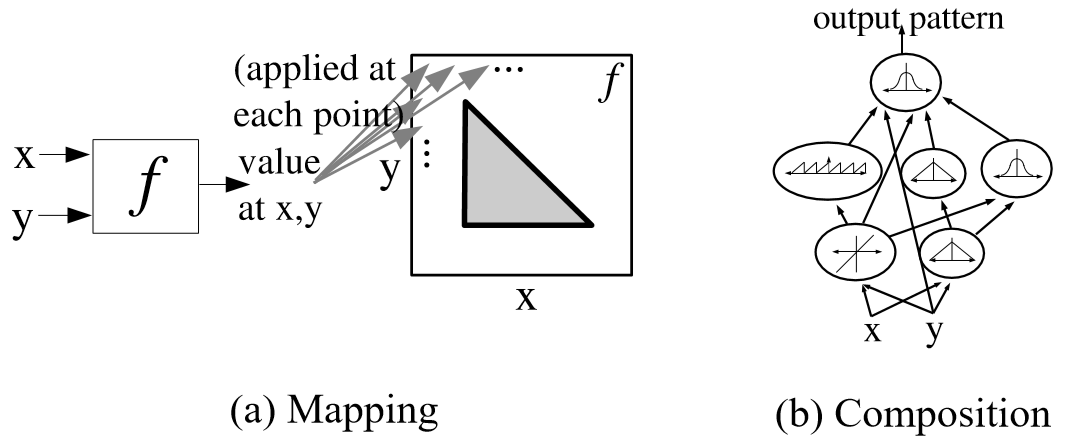
\includegraphics[width=0.7\linewidth]{figures/HyperNeat/CPPN}
	\caption[Exemplar CPPN]{(a) The mapping of a function f from a two dimensional connection space to a one dimensional spatial pattern. x and y are the positions of two neurons. (b) f's internal structure called a CPPN is shown. The output is a composition of different basic functions in a network. The connections in the CPPN are weighted such that the output of a function by the weight of it's outgoing connection. \cite[p. 5]{HyperNEAT}}
	\label{fig:cppn}
\end{figure}

\begin{figure}[tb]
	\centering
	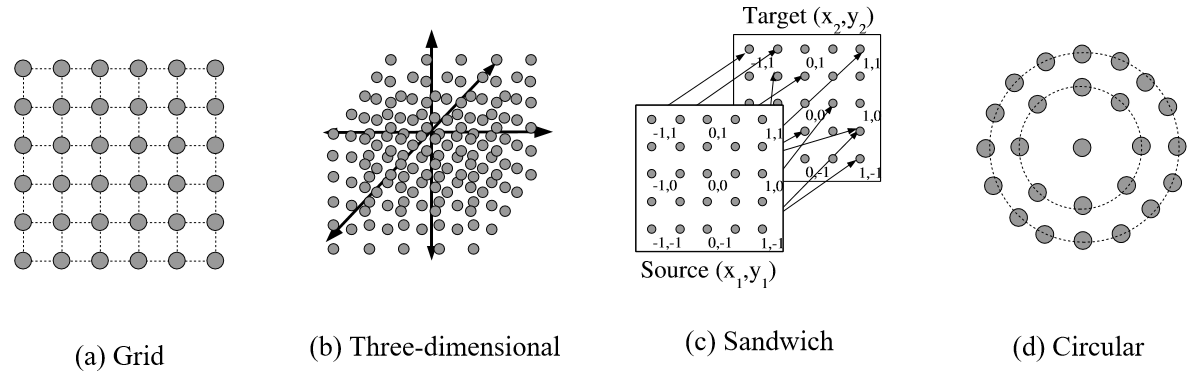
\includegraphics[width=0.7\linewidth]{figures/HyperNeat/Substrates}
	\caption[Exemplar Substrate Configurations]{ Examples of how to define a substrate configuration. That is how to arrange the position of neurons. They can be of different dimensions and described by different coordinate systems. (a),(b) and (c) are in Cartesian coordinates while (d) is represented in polar coordinates. (a) and (d) are one dimensional while (b) is three dimensional. (c) is an implicit three dimensional case, where the third dimension is ignored. In this case all input neurons lay on a different layer in 3D space than the output neurons. Note that self linked neurons are not possible in this scenario. Substrates describe the geometric relationship of neurons, so different substrates are suited for problems with different geometric properties.
	\cite[p. 11]{HyperNEAT}}
	\label{fig:substrates}
\end{figure}



\begin{figure}[tb]
	\centering
	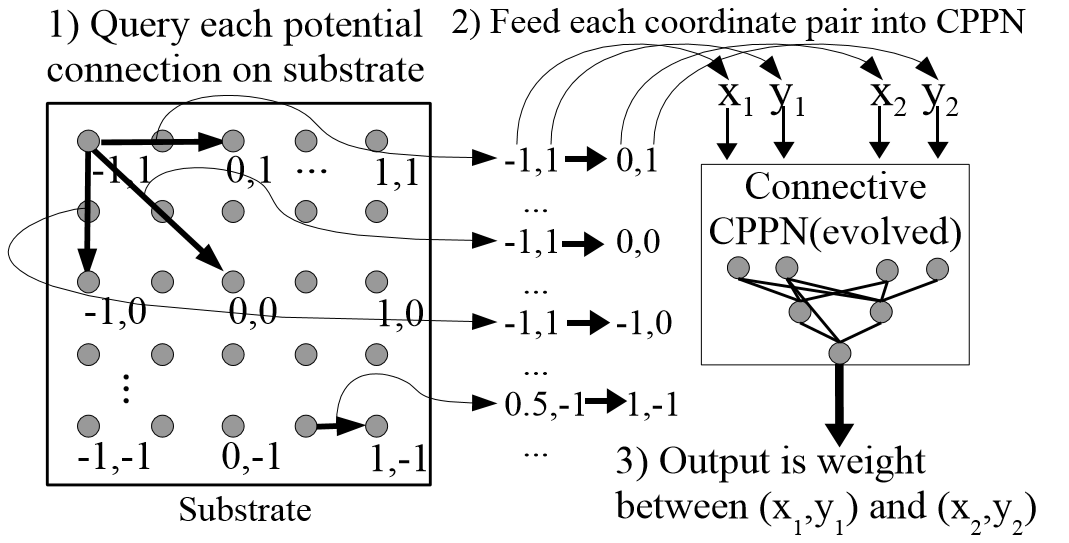
\includegraphics[width=0.7\linewidth]{figures/HyperNeat/QuerySubstrate}
	\caption[ANN creation with HyperNEAT]{This figure shows how a ANN is created by HyperNEAT. The coordinates of each pair of nodes (potential connection) are applied to the CPPN. A pair of nodes is depicted by a black arrow. If the CPPN's output is higher as a defined threshold (not depicted) a weighted connection between those two nodes is created. In this example a two dimensional grid substrate and thus a CPPN with four inputs is used. 	\cite[p. 9]{HyperNEAT} }
	\label{fig:querysubstrate}
\end{figure}


\begin{figure}[tb]
	\centering
	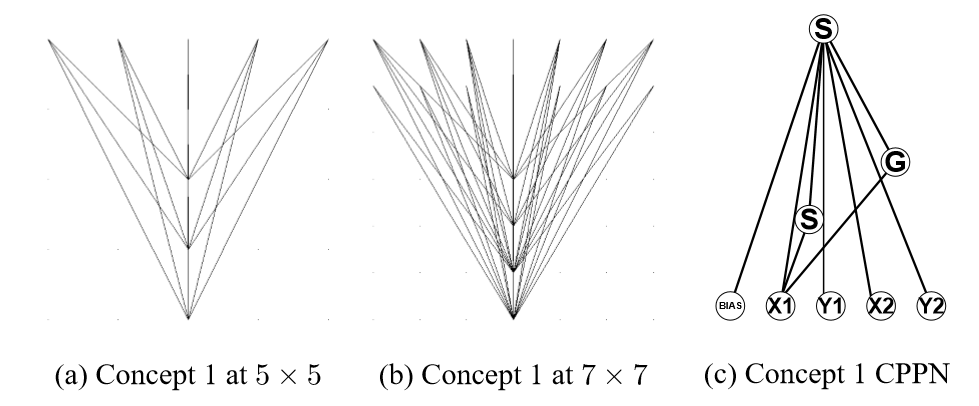
\includegraphics[width=0.7\linewidth]{figures/HyperNeat/scaling}
	\caption[Exemplar substrate scaling]{ The spatial pattern produced the CPPN on the right (c) can be queried by different substrates. (a) shows the resulting network of a 5 x 5 grid substrate and (b) the resulting network of a 7 x 7 grid substrate on the same space. From (a) to (b) the substrate was even scaled by factor $1.4$.  \cite[p. 14]{HyperNEAT}}. The CPPN activation functions are denoted by G for Gaussian and S for sigmoid.
	\label{fig:scaling}
\end{figure}

Scaling:\\
 \cite{HyperNEAT} and \cite{HyperNEATOctobusArm} argue that the spatial pattern produced by a CPPN encodes a general connectivity concept. Based on this statement they show empirically that the resolution of a substrate configuration can be changed to vary the size of the resulting ANN with only minor influences on the result. For example instead of an $5x5$ grid substrate configuration one could scale the substrate configuration to a $7x7$ grid substrate applied to the same space (e.g $[0,1]$). This process is further on referred as substrate scaling. One benefit of substrate scaling is, that one can scale the resulting with use of the same substrate without further evolution needed. Example solution of a scaled substrate configurations are shown in figure \ref{fig:scaling}.
 
 CPPN configuration variation: \\
 \cite{HyperNEATOctobusArm}, \cite{HyperNEATLeo},\cite{HyperNEATEvolveLearningRules} and \cite{HyperNeat1DSubstrates} varied the number of inputs and outputs of the CPPN to encode further information than the neuron position. \cite{HyperNEATLeo} decouples the weight and the expression of a connection. He defines with the value of a second output whether the connection is evolved or not. One other variation from \cite{HyperNEATOctobusArm}  is two have three layered sandwich substrate configuration where the second CPPN output defines the connections between the second and third layer.\cite{HyperNEAT} adds an additional input node to additionally decode the distance between the geometric distance between the two nodes. Further on one can use a additional bias neuron wit a constant input as input neuron as \cite{HyperNEATEvolveLearningRules} did. TODO draw own picture with those variations.  \cite{HyperNEATLeo} states that Hyperneat "tends to generate fully connected networks" and shows that due to the separation of weight encoding and connectivity expression less connected modular networks can evolve.
 
Placement without geometric relationship:\\
  (\cite{HyperNEATUnknownGeometry}) deals with the problem that it is hard to place neurons if there is no clear geometric relationship between them. A first approach would be to put each logical group as one line into a 2D space. This approach has the problem that HyperNEAt has to detect and find a complex function to distinguish between the logical groups. Therefore \cite{HyperNEATUnknownGeometry} suggestes to minimize the geometrical dependencies by grouping logically related neurons in own spaces and than creating a multi level sandwich structure. For each two connected spaces an additional CPPN output is created. This CPPN structure gives hyperNEAT a structural hint that logical groups exist and simple connectivity patterns between each group can be found and relationships between them encoded by the CPPN. An example of this approach is depicted in picture \ref[p 4]{fig:nogeometricrelationship}.
  
\begin{figure}[tb]
	\centering
	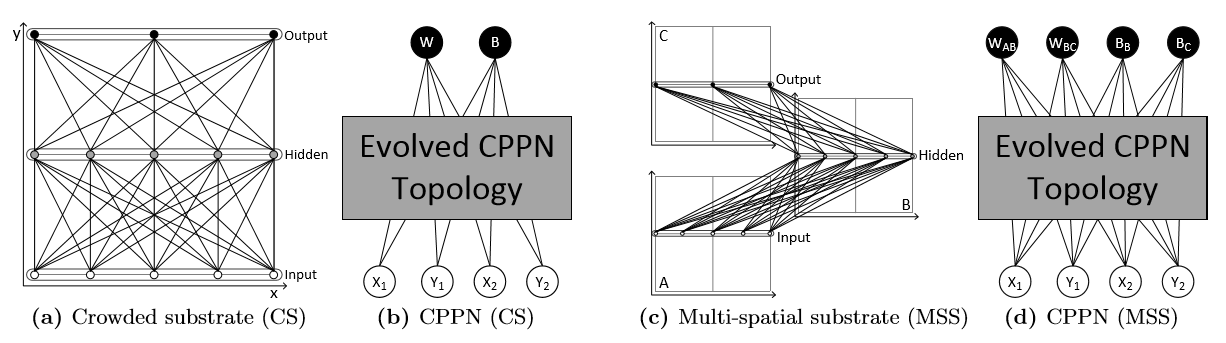
\includegraphics[width=0.7\linewidth]{figures/HyperNeat/noGeometricRelationship}
	\caption[HyperNEAT no geometric relationships]{\textbf{HyperNEAT with no geometric relationships}. The shown output hidden and input neurons have only logical dependencies but no geometric ones. Substrate configuration (a) with CPPN (b) show an approach that forces HyperNEAT to find a complicated function to distinguish the logical groups. By creation of an own space for each logical group which leads to a sandwich structure (c) and additional CPPN outputs (b) describing the spatial pattern between two spaces. With this approach simple connectivity patterns can be found. Note that in approach (c,d) a one dimensional neuron space would be sufficient.  The output neurons $B$,$B_B$ and $B_C$ are not relevant for this example. \cite{HyperNEATUnknownGeometry}}
	\label{fig:nogeometricrelationship}
\end{figure}
  TODO argue like him why 1d hyperneat has this extension..
 
 

 Wichtig, gutes zitat irgendwo verwenden:
 \cite{HyperNEATLeo} states that Hyperneat "tends to generate fullyconnected networks"

 Scaling: TDDO 
 CPPN configurations: multiple input, outputs
 Modulationary CPPNs:
 
 
 zitiere checkers game, robot arms, b

TODO mention much lower search space in cppn.


substrate = output of cppn
or substrate = placement of neurons.
or substrate = resulting network !!
Ok last one gives most sense!!

TODO draw retina example.

-> senstifity to chosen geometrie -> Paper (The Sensitivity of HyperNEAT to Different Geometric Representations of a Problem)

Hypercube-based NeuroEvolution of Aug
menting Topologie
\subsection{ES-HyperNEAT}\label{ES_HYPERNEAT}
Since Hyperneat (see section \ref{HYPERNEAT}) is only able to optimize the connections of an ANN it lacks the ability to vary the amount of neurons. Evolvable Substrate HyperNEAT (ES-Hyperneat) (see generally \cite{ESHyperNEATarticle}, \cite{ESHyperNEATPaper} ) provides a method based on HyperNEAT that has the ability to evolve the whole topology of a network including neurons, their location in space, connections and weights. 
The basic idea of ES-HyperNEAT is that each band of equal weights in the spatial pattern defines connections. Since 
The basic idea of ES-HyperNEAT is that points in a spatial pattern created by a CPPN represent connections and that those connections are selected from bands of equal weights. This procedure basis on the fact, that information is defined by variance. So at regions with a high variance density many bands are found and thus many connections are evolved. At regions with a low variance density less bands are found and thus less connections are evolved. Since a connection is represented by a point in connection space witch is double the dimension of the neuron space, a connection two neurons and the coordinates of those. As in HyperNEAT (section \ref{HYPERNEAT}) the connections weight is derived by the value of the spatial pattern at the connection's coordinates.\\
The connection space used in ES-HyperNEAT is 4 dimensional. But, because the search for variances in the four dimensional space is expensive, Es-HyperNEAT searches for connections by starting from the input nodes. The coordinates of the input node are fixed in the 4D connection space. As a result a 2 dimensional cross section of the hypercube is considered, which describes outgoing connections from the input node. The coordinates of the point from which new connections are searched are denotes as $(a,b)$. further on.
To determine bands in the connection space a quadtree based "division and initialization phase" is applied. And followed by a "pruning and extraction phase". 
In the "division and initialization phase" a quadtree is laid recursively over the cross section of the connection space. Each node describes a square and has 4 children as long it's not a leaf node. The parent node spans a square from $(-1,-1)$ to $(1.1)$. It has 4 children describing 4 equal spaced subsquares of the parent's square. The initial resolution $r$ defines the minimal depth of the tree: Minimal depth $= \sqrt{r}+1$. (e.g a initial resolution of 16 leads to $16x16$ squares and a depth of 4). The centre point $(x,y)$ of each square describes a potential connection. It's weight is determined by querying the CPPN with arguments $(a,b,x,y)$. The weight variance of each tree node $p$ is calculated as $\sigma^2_p = \dfrac{1}{k}\displaystyle\sum_{i=1}^{k} (\overline{w}-w_i)^2)$. Where $k$ is the amount of leaf nodes of the subtree of p. $\overline{w}$ describes the median weight over all leaf nodes' weights. Note that the variance of a leaf note is $0$. $\sigma^2_p$ is an indicator for the variance of the spatial pattern at this square. If the weight variance of a leaf node's parent is higher a given division threshold $d_t$ division and initialization phase is reapplied starting from the parent's square. This gives the quadtree the possibility to create more nodes at areas with higher variance. However the total depth of the quadtree is bounded by a maximum resolution level $r_m$.
In the following "pruning and extraction phase" connections are chosen out of the potential connections describe by the quadtree. 
Firstly a depth first search is applied to the quadtree. If a node's parent's variance is smaller than a given variance threshold $\sigma^2_t$ a connection $(a,b,x,y)$ is created. $x,y$ are the coordinates of the current node. In a second since we only want to have the connections clearly inside a band the connections at the edges are deleted. To do so only connections (=squares) are kept whose point of two neighbouring squares of he same size on opposite sides (left and right, or top and bottom) differ in weight. The weight difference $\beta$ also called band level has to be higher than a given band threshold $\beta_t$. $\beta$ is defined as follows:
\label{lbl:weight difference}
\begin{align*}
	\beta &= \max(\min(d_{top},d_{bottom}),\min(d_{left},d_{bottom}))\\
	d_{top} &= |CPPN(a,b,x,y)-CPPN(a,b,x,y+m)|
\end{align*}  
$d_{bottom}$,$d_{left}$,d$_{bottom}$ are calculated accordingly to $d_{top}$. $x,y$ are the coordinates of the centre point of the current square and $m$ the widths of the current square.
Own additions:
As a result considering two a narrow and a wide band of same length the more narrow one will have more neurons since a higher resolution of the quadtree is needed to define squares in the band. Thus the existing of neurons  in a band depends on whether it's variance is over the variance threshold. The number of neurons on created on the band depends on the width and length of the band.(not own) The total amount of neurons can be increased either by adding more bands or by making them thinner.
The frame of the whole ES-HyperNEAT algorithm doesn't change much compared to the HyperNEAT algorithm. The whole evolution process keeps the same. It differs only in the way the ANN is build out of the CPPN(genome). The positions of  input and output neurons must be given. Now starting with input neurons for each neuron the "division and initialization phase" and "pruning and extraction phase" are applied. For every found connection the corresponding hidden neuron is created if not already existing. Now this concept is applied again on all new found neurons. This gets repeated until an given maximum iteration level $it_{max}$ is reached. To find connections between the output neurons and all other neurons again cross section of the Hypercube are created. But this time with fixed output coordinates. That is $w=CPPN(x,y,a,b)$. After all neurons and connection have been found all neurons and connections that are not on a path from an input to an output neuron are deleted.
To sum up the ES-HyperNEAT Algorithm is shown below:

	\SetCommentSty{text} 
\begin{algorithm}[h!] % or H with float
	\label{ES-HyberNEATAlgorithm}
	\TitleOfAlgo{ES-HyperNEAT algorithm}
	choose strategy parameters\;
	define input and output neuron positions
	create initial population P(0) with minimal CPPNs and random weights\;
	$t \gets 0$\;
	evaluate fitness of the initial population \tcp*[r]{like it is done below}
	\While{termination condition not reached}{
		$t \gets t+1$\;
		\ForAll(\tcp*[f]{genome = CPPN}){genomes in P(t)}{ 
			$unvisitedNeurons \leftarrow inputNeurons$
			$neurons\leftarrow \leftarrow inputNeurons$
			$connections\leftarrow \emptyset$
			\For{i=0 \KwTo $iterationLevel$)}{ 
				$newNeurons \leftarrow \emptyset$
				\ForEach{$node \in unvisiteNeurons$}{
					\tcp*[f]{division and initialization phase} \\
					build quadtree on cross-section of the hypercube\;
					\tcp*[f]{pruning and extraction phase}\\
					prune and express new connections   
					\ForEach{new connection}{
					get coordinates of $newNeuron$\;
					\If{$newNeuron \notin neurons$}{$newNeurons \leftarrow  (newNeurons \cup newNeuron) $}
					} 
					$neurons \leftarrow neurons \cup newNeurons$\;
					$connections \leftarrow connections \cup newConnections$\;
		     	}
	     		$unvisitedNeurons \leftarrow  newNeurons$\;
			}
			express connections from $outputtNeurons$ to $neurons$\tcp*[r]{like it is done above but without note expression and CPPN(x,y,a,b)}
			$neurons \leftarrow neurons \cup outputNeurons$\;
			Delete all neurons and connections that are not on a path between an input and an output neuron.\;
			
			Build ANN out of $neurons$ and $connections$\;
			Determine fitness of created ANN\;
		}
		create new population P(t) with NEAT\;
	}
	output best CPPN;
	%\ similar in modularity paper
	%\caption{How to write algorithms}
\end{algorithm}
For better clarity all ES-HyperNEAT parameter are listed again in \ref{table:ES-HYPERNAET-Params}.
TODO algorithm and plots.



\begin{figure}[tb]
	\centering
	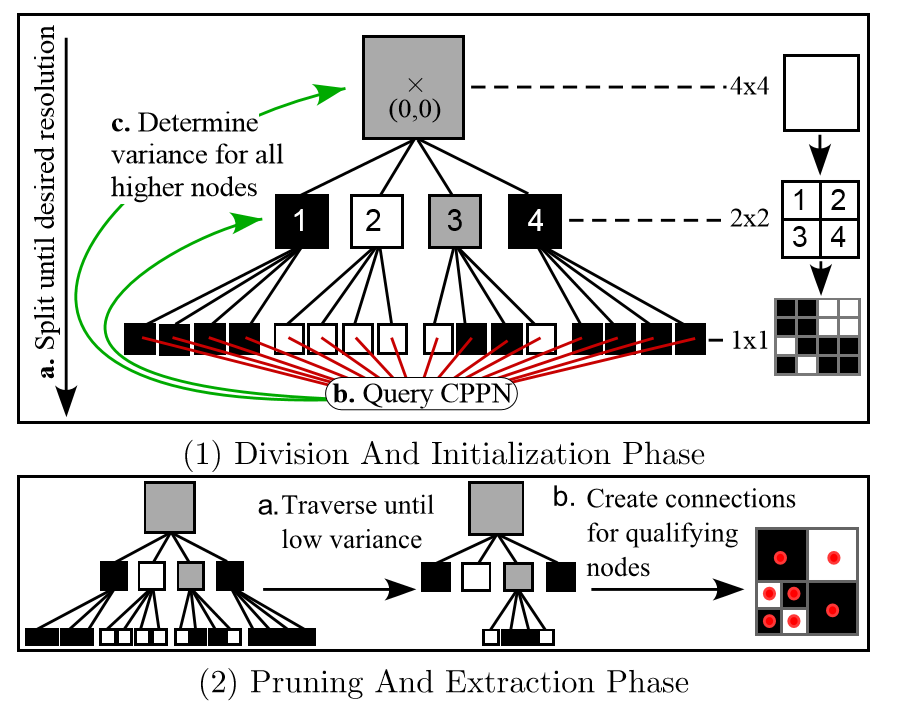
\includegraphics[width=0.7\linewidth]{figures/ES-HyperNEAT/Es-HyperNEATPhases}
	\caption[ES-HyperNeat Phases]{\textbf{ES-HyperNeat Phases}. This figure shows the division and initialization phase as well as parts of the pruning and extraction phase. Note that band pruning is not depicted. Gray squares indicate a weight variance higher than the variance threshold but lower then the division threshold. Black and white squares have weight variances of 0. The initial resolution is 16. As first step in the first phase a quadtree with the minimal solution is created (1a), then the CPPN values at the centre of each leave nodes' square are queried(1b). Based on these values, the variance of each non leaf node is calculate(1c). Since no node has a higher weight variance than the division threshold no further and deeper nodes are created. In the second phase a depth first search is applied only extraction childs of nodes whose variance is higher than the variance threshold(2a). Here the children of node 1,2 and 4 are not expressed because their variance is 0. For each remaining leaf node a connection is created (2b). \cite[p. 14]{ESHyperNEATarticle} }
	\label{fig:es-hyperneatphases}
\end{figure}




\begin{figure}[tb]
	\centering
	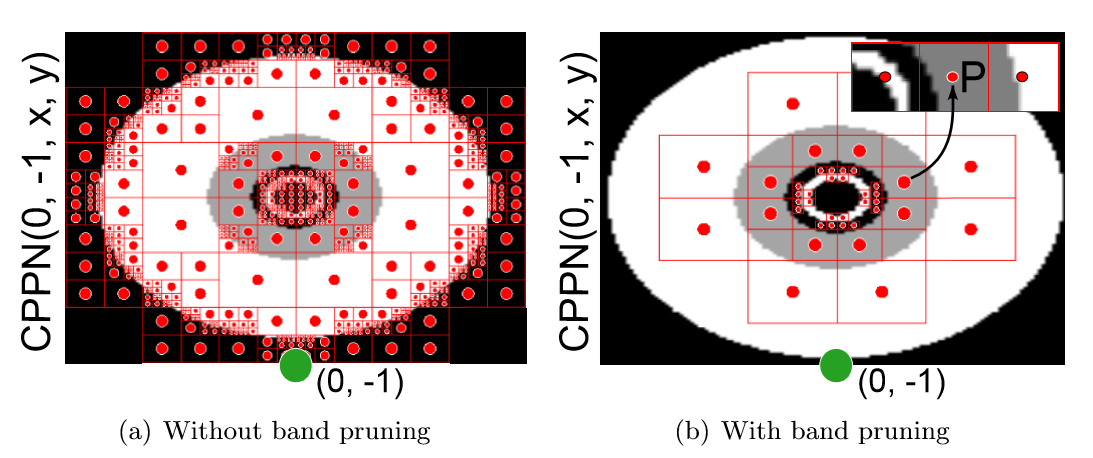
\includegraphics[width=0.7\linewidth]{figures/ES-HyperNEAT/ES-HyperNeatBandPruning}
	\caption[ES-HyperNeat band pruning]{\textbf{ES-HyperNeat band pruning}. The background of both images shows a 2d slice of a 4D hypercube. The slice is created by querying a CPPN with fixed input neuron positions (0,-1).Different grey scale values represent different CPPN output values. (a) shows the intermediate result of the "pruning and extraction phase" before band pruning is applied. All found points(=connections) indicate the variance of the CPPN output. In "band pruning" (b) only points are kept that are enclosed by two neighbours on opposite sides at the same resolution with different CPPN values (e.g point P). As a result only points inside a band and not at the edge are left. Those points represent the information about the ANN inherent in a slice of a spatial pattern. \cite[p. 15]{ESHyperNEATarticle}}
	\label{fig:es-hyperneatbandpruning}
\end{figure}


\begin{figure}[tb]
	\centering
	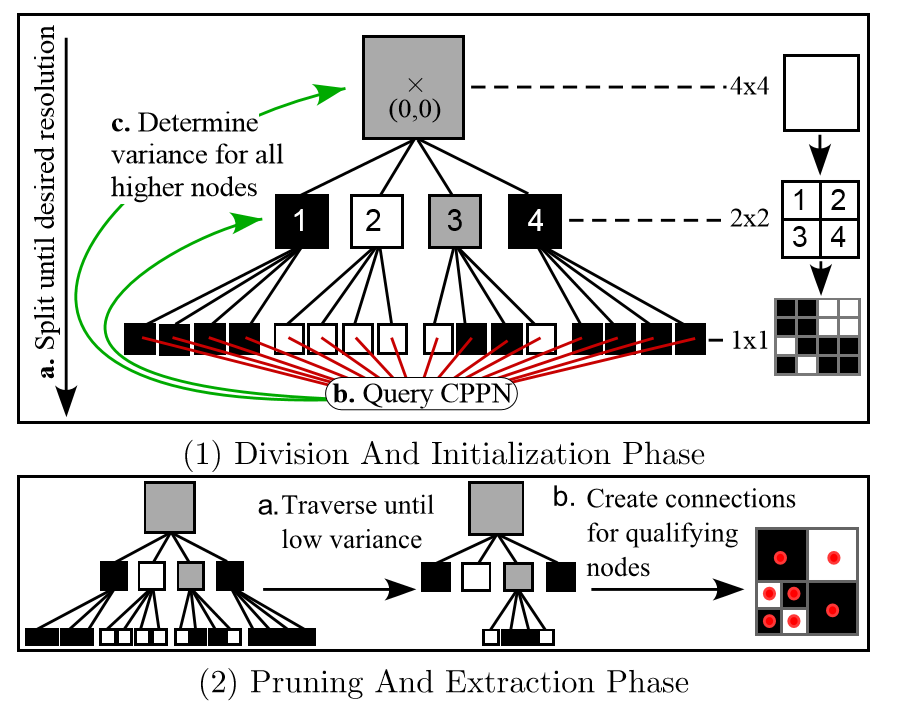
\includegraphics[width=0.7\linewidth]{figures/ES-HyperNEAT/Es-HyperNEATPhases}
	\caption[ES-HyperNeat algorithm]{\textbf{ES-HyperNeat algorithm scenario}.In this scenario the ES-HyperNeat algorithm starts with querying the slice of the Hyperspace created by fixing the input position parameters to the position of the input neuron (CPPN(0,1,x,y))(a). Note that each found neuron (red points) lay inside a band. Now slices for each hidden node position are queried and new connections and nodes created (b). To determine the connections to the output neuron. The output position parameters of the CPPN are fixed to the position of the output neuron (CPPN(x,y,0,1)). In this case no new nodes but only connections are created. To construct a sense full ANN only those neurons and connections are kept that are part of a path from the input to the output neuron (d). \cite[p. 17]{ESHyperNEATarticle}}
	\label{fig:es-hyperneatphases}
\end{figure}

hyperneat better in modularity. Emperically shown in multimodal environment

\begin{table}[h]

\begin{tabular}{ l | l | l }		
	parameter & nomination & description \\
	\hline
	$r$ & initial resolution & minimal number of leaf nodes in the quadtree \\
	$r_m$ & maximum resolution & maximal number of leaf nodes in the quadtree  \\
	$\sigma^2_p$ &  weight variance of node p & an indicator of the real variance of the function in the square described by p.\\
    $d_t$ & division threshold& if a node's variance is higher than the division threshold it's children are realized As long $r_m$ is not reached.\\ 
	$\sigma^2_t$&variance threshold& minimal variance a node must have that its children's connections are realized\\ 
    $\beta_t$& band threshold & determines upon the weight difference $\beta$ (see \ref{lbl:weight difference}), whether a point is inside a band or not.\\
    $it_{max}$&maximum iteration level& determines how often all in one iteration found hidden nodes are scanned again for new nodes.
\end{tabular}
\caption[ES-HyperNEAT parameter overview ]{ES-HyperNEAT parameter overview}
\label{table:ES-HYPERNAET-Params}
\end{table}

TODO add algotihm from paper not article. vielleicht wenn unvrständlich.
TODO text dazu anpassen.  replace weight with CPPN value
TODO band pruning and pruning , ne passt so.

Zitat:"
Density
follows information" mit density meint er die neuronendichte
His description that a uniform gradient computes the same function at every point (what is right) is bad, is questionable. Also a fully connected net with higher or less resolution might work well !  p.11



\section{Motorcortex Model}\label{MotorCortex_Model}

%%% Introduction
%%%%%%%%%%%%%%%%%%%%%%%%%%%%%%%%%%%%%%%%%%%%%%%%%%%%%%%%%%%%%%%%%%%%%
% Einleitung
%%%%%%%%%%%%%%%%%%%%%%%%%%%%%%%%%%%%%%%%%%%%%%%%%%%%%%%%%%%%%%%%%%%%

\chapter{Introduction}\label{Introduction}

Start with a comprehensive introduction about the questions of your thesis.

The thesis could include a background section, which also could become one or two separate chapters.

Do not forget to also give a short overview of the structure of the thesis in this chapter, for example as follows:

\medskip
This thesis is structured as follows: First a background on XXX is introduced in the following background chapter (or the following section).
In chapter~\ref{MetMat} the developed algorithm to analyse ... is presented, followed by a comprehensive description of the used data or material.
The results are given in chapter~\ref{results}. A discussion and short outlook conclude this thesis.

The following (in german) help newbies in \LaTeX to learn about sections, math equations and much more.

Bevor wir uns der Auswertung bzw. Bewertung der gewonnenen Prim\"ardaten zuwenden, wollen wir zun\"achst einige grundlegende Begriffe der deskriptiven Statistik wiederholen.
\section{Stichproben}

Grunds\"atzlich haben wir es bei Microarrayexpressionsdaten mit einer {\em Stichprobe} aus einer {\em Population (Grundgesamtheit)} zu tun.   
Wir bezeichnen nun im allgemeinen mit $X=\{x_1,x_2,\ldots,x_n\}$ die Beobachtungsdaten vom Umfang $n$. 
Diese Daten sollen mit statistischen Kenngr\"o\"sen beschrieben werden. Aus diesen will man m\"oglichst zuverl\"assig auf die zugrundeliegende Verteilung in der Grundgesamtheit schlie\"sen. Hierzu verwenden wir die {\bf Lage-} und {\bf Streuparameter}. Zun\"achst wenden wir uns aber der H\"aufigkeits- und Summenh\"aufigkeitsverteilung zu, die sowohl graphisch als auch numerisch einen Eindruck \"uber die Verteilung von $X$ bieten. Daf\"ur betrachten wir diskrete Verteilungen.

Gegeben sei eine Stichprobe $(X_1,X_2,\ldots,X_n)$. Eine Funktion $Z_n=Z(X_1,\ldots,X_n)$ heisst eine {\em Stichprobenfunktion}. Sie ist selber eine Zufallsgr\"o\"se.

\subsection{H\"aufigkeiten und Histogramm}
In $X$ trete der Wert $x_i$ genau $n_i$ mal auf, $i=1,2,\ldots m$. Dann ist $\sum_i n_i = n$. Der Quotient $n_i/n$ ist die {\em relative H\"aufigkeit} f\"ur das Eintreten des Ereignisses ``$X=x_i$''.
Die Menge der relativen H\"aufigkeiten $\{n_1/n,n_2/n,\ldots, n_m/n\}$ hei\"st {\em H\"aufigkeitsverteilung} von $X$. Ferner hei\"st die Menge $\{s_1,\ldots,s_m\}$ mit $s_i=\sum_{k=1}^{i}n_k/n$ die {\em Summenh\"aufigkeitsverteilung} von $X$.

F\"ur die graphische Darstellung der H\"aufigkeitsverteilung wird das {\em Histogramm} (s. Abb.~) gew\"ahlt. f\"ur die Summenh\"aufigkeitsverteilung die {\em Treppenfunktion}.

%
\subsection{Wichtige Verteilungen}

\subsubsection{Die Normalverteilung}
Die Dichte der Normalverteilung ist gegeben durch
\begin{equation}\label{dichtenormal}
g(x) = \frac{1}{2\pi\sigma}\cdot e^{-\frac{(x-\mu)^2}{2\sigma^2}}
\end{equation}
wobei $\mu$ (Lage) der Mittelwert und $\sigma$ (Breite) die Standardabweichung der Normalverteilung ist. 
Durch die $z$-Transformation l\"asst sich die Normalverteilung auf die Standardnormalverteilung mit $\mu=0$ und $\sigma=1$ transformieren.

Die Normalverteilung bildet die Basis fast der gesamten statistischen Theorie. \footnote{ 
``Everyone believes in the normal law, the experimenters because they imagine it is a mathematical theorem, and the mathematicians because they think it is an experimental fact.'' (Gabriel Lippman, in Poincar\'e's Calcul de probabilit\'es, 1896)}. Auch bei der Analyse der Microarraydaten werden wir sehr oft von der Annahme der Normalverteilung Gebrauch machen. Allerdings sollten wir uns klarmachen, dass  rein experimentell zahlreiche Untersuchungen gezeigt haben, dass die echten Fehler selten, wenn \"uberhaupt normal verteilt sind.


\section{Sch\"atzung von Parametern}
Allgemein erhofft man sich beim Ziehen einer Stichprobe, einen unbekannten Parameter $\gamma$ der Grundgesamtheit, z.B. den Mittelwert, aus der Stichprobe zu sch\"atzen.
\subsection{Eigenschaften von Punktsch\"atzungen}


%\cleardoublepage
%
%%% 
%%%%%%%%%%%%%%%%%%%%%%%%%%%%%%%%%%%%%%%%%%%%%%%%%%%%%%%%%%%%%%%%%%%%%
% Grundlagen
%%%%%%%%%%%%%%%%%%%%%%%%%%%%%%%%%%%%%%%%%%%%%%%%%%%%%%%%%%%%%%%%%%%%

\chapter{Methods and Material}
  \label{MetMat}

\noindent
Ziel dieses Kapitels ist eine Einf\"uhrung in die Thematik BlaBlaBla ...

\section{title of section}
  \label{Abschnittslabel} 

BlaBlaBla ...

\subsection{title of subsection}
  \label{Unterabschnittslabel}

BlaBlaBla ...

Im folgenden wird das Einbinden einer Abbildung als `pdf-Datei' in ein
\LaTeX-Dokument gezeigt.

\begin{figure}[htb]
     \centerline{\epsffile{figures/chordal.eps}}
  \caption{Chordale Graphen}
  \label{fig2.1}
\end{figure}

Abbildung~\ref{fig2.1} zeigt ...

Tabellen k\"onnen wie folgt erstellt werden:

{
\renewcommand{\baselinestretch}{0.9} 
\normalsize
\begin{table}[htb]
\begin{tabular}{|p{2.7cm}||l|c|r|}
\hline
    \textbf{Spalte 1} 
  & \textbf{Spalte 2} 
  & \textbf{Spalte 3} 
  & \textbf{Spalte 4} \\
  \hline\hline
  xxx1111
  & xxxxxxx2222222
  & xxxxxx333333 
  & xxxxxxxxxx444444 \\
  \hline
    ...
  & ...
  & ...
  & ...\\
  \hline
\end{tabular}
  \caption[Beispieltabelle mit einer langen Legende]{Beispieltabelle mit einer langen Legende, damit man sieht, dass in der Legende der Zeilenabstand verringert wurde. Ausserdem soll auch der Font etwas kleiner gew\"ahlt werden. So sieht die ganze Umgebung kompakter aus.}
  \label{tabelle-1}
\end{table}
}

\noindent
Eine Aufz\"ahlung geht wie folgt:
\begin{itemize}
\item ...
\item ...
\end{itemize}
Eine numerierte Aufz\"ahlung:
\begin{enumerate}
\item ...
\item ...
\end{enumerate}

Betonungen sollen \emph{kursiv} gedruckt werden. 
\textbf{Fettdruck} ist auch m\"oglich.

Referenzen: \cite{SaaSchTue97,TueConSaa96ismis,SchTueSaa98preprint}

%\cleardoublepage
%
%%%
%%%%%%%%%%%%%%%%%%%%%%%%%%%%%%%%%%%%%%%%%%%%%%%%%%%%%%%%%%%%%%%%%%%%%
% Diskussion und Ausblick
%%%%%%%%%%%%%%%%%%%%%%%%%%%%%%%%%%%%%%%%%%%%%%%%%%%%%%%%%%%%%%%%%%%%

\chapter{Results}
  \label{results}

In this chapter which also could be more than one chapter, depending on the nature of the thesis, the results of the thesis are presented.
Make sure you illustrate your results with appropriate figures and tables, but do not discuss the results here.This should be done in a separate discussion chapter.

\clearpage

%\cleardoublepage
%
%%%
%%%%%%%%%%%%%%%%%%%%%%%%%%%%%%%%%%%%%%%%%%%%%%%%%%%%%%%%%%%%%%%%%%%%%
% Diskussion und Ausblick
%%%%%%%%%%%%%%%%%%%%%%%%%%%%%%%%%%%%%%%%%%%%%%%%%%%%%%%%%%%%%%%%%%%%

\chapter{Discussion and Outlook}
  \label{Discussion}

Of course very important! You need to discuss the informatics as well as bio part of your thesis topic.

\bigskip
Take your time for writing the discussion, besides the introduction chapter it is the most important chapter of your thesis.
Also do not subsection the discussion too heavily.
\clearpage
At least 5 pages.
\clearpage
Outlook can become an extra chapter.

%\cleardoublepage
%
%
%%%%%%%%%%%%%%%%%%%%%%%%%%%%%%%%%%%%%%%%%%%%%%%%%%%%%%%%%%%%%%%%%%%%%%%%%%%%%%
%%%% Appendix
%%%%%%%%%%%%%%%%%%%%%%%%%%%%%%%%%%%%%%%%%%%%%%%%%%%%%%%%%%%%%%%%%%%%%%%%%%%%%%

% used parameters, neat, Hyperneat, Model sebastian 

%\appendix
%
%%\setcounter{secnumdepth}{-1}
%%\section{Tables}\label{chap:App}
%\chapter{Further Tables and Figures}\label{chap:App}
%Viele Arbeiten haben einen Appendix. Besondere Sorgfalt muss beim Nummerieren der Tabellen und Abbildungen gewährleistet sein.
%\begin{table}[htb]
%\begin{tabular}{cc}
%Nummer & Datum \\
%\hline
%1 & 1.1.80\\
%2 & 1.1.90 \\
%\end{tabular}
%\caption{Erste Appendix-Tabelle}\label{tab:app1}
%\end{table}
%
%%\chapter{Figures}\label{chap:App2}
%
%\begin{table}[htb]
%\begin{tabular}{cc}
%Nummer & Datum \\
%\hline
%1 & 1.1.80\\
%2 & 1.1.90 \\
%\end{tabular}
%\caption{Zweite Appendix-Tabelle}\label{tab:app2}
%\end{table}
%%\end{appendices)
%
%\cleardoublepage
%
%%%%%%%%%%%%%%%%%%%%%%%%%%%%%%%%%%%%%%%%%%%%%%%%%%%%%%%%%%%%%%%%%%%%%%%%%%%%%
%%% Bibliographie
%%%%%%%%%%%%%%%%%%%%%%%%%%%%%%%%%%%%%%%%%%%%%%%%%%%%%%%%%%%%%%%%%%%%%%%%%%%%%

\addcontentsline{toc}{chapter}{Bibliography}

\bibliographystyle{alpha}
\bibliography{mylit}
%% Obige Anweisung legt fest, dass BibTeX-Datei `mylit.bib' verwendet
%% wird. Hier koennen mehrere Dateinamen mit Kommata getrennt aufgelistet
%% werden.

\cleardoublepage
%%%%%%%%%%%%%%%%%%%%%%%%%%%%%%%%%%%%%%%%%%%%%%%%%%%%%%%%%%%%%%%%%%%%%%%%%%%%%%
%%%% Erklaerung
%%%%%%%%%%%%%%%%%%%%%%%%%%%%%%%%%%%%%%%%%%%%%%%%%%%%%%%%%%%%%%%%%%%%%%%%%%%%%%
%\thispagestyle{empty}
%\section*{Selbst\"andigkeitserkl\"arung}
%
%Hiermit versichere ich, dass ich die vorliegende Masterarbeit 
%selbst\"andig und nur mit den angegebenen Hilfsmitteln angefertigt habe und dass alle Stellen, die dem Wortlaut oder dem 
%Sinne nach anderen Werken entnommen sind, durch Angaben von Quellen als 
%Entlehnung kenntlich gemacht worden sind. 
%Diese Masterarbeit wurde in gleicher oder \"ahnlicher Form in keinem anderen 
%Studiengang als Pr\"ufungsleistung vorgelegt. 
%
%\vskip 3cm
%
%Ort, Datum	\hfill Unterschrift \hfill 
%%%%%%%%%%%%%%%%%%%%%%%%%%%%%%%%%%%%%%%%%%%%%%%%%%%%%%%%%%%%%%%%%%%%%%%%%%%%%%
%%%% Ende
%%%%%%%%%%%%%%%%%%%%%%%%%%%%%%%%%%%%%%%%%%%%%%%%%%%%%%%%%%%%%%%%%%%%%%%%%%%%%%

\end{document}

